\documentclass[11pt, oneside]{article}   	% use "amsart" instead of "article" for AMSLaTeX format
\usepackage{geometry}                		% See geometry.pdf to learn the layout options. There are lots.
\geometry{letterpaper, margin=1.0in}                   		% ... or a4paper or a5paper or ... 
%\geometry{landscape}                		% Activate for rotated page geometry
\usepackage[parfill]{parskip}    		% Activate to begin paragraphs with an empty line rather than an indent
\usepackage{graphicx}				% Use pdf, png, jpg, or eps§ with pdflatex; use eps in DVI mode
								% TeX will automatically convert eps --> pdf in pdflatex		
\usepackage{amssymb}
\usepackage{hyperref}
\usepackage{comment}
\usepackage[dvipsnames]{xcolor}
%SetFonts

%SetFonts


\title{Circumgalactic dust halos update \#2}
\author{Jacqueline McCleary}
%\date{}							% Activate to display a given date or no date

\newcommand{\dMdp}{\rm \frac{\partial M}{\partial \rho}} 
\newcommand{\dMinline}{$\rm \partial M / \partial \rho$~}
\newcommand{\av}{$A_V$~}

\begin{document}
\maketitle

%%%%%%%%%%%%%%%%%%%%%%%%%
%%%
%%% SECTION: Overview
%%%
%%%%%%%%%%%%%%%%%%%%%%%%%

\section{Executive Summary}

This is a short follow-up to the comprehensive ``Circumgalactic dust halos update'' document circulated in October 2023. Here are the principal updates since that time: 

\begin{enumerate}
\item Implemented redshift-based matching for augmenting redMaGiC random catalogs with galaxy colors (see Figure \ref{fig:redshiftmatch}. This change did not visibly affect extinction profiles.  
\item Fixed a bug in the generation of random (foreground) catalogs; my previous algorithm, which randomly sampled HEALPixels and then calculated the central RA and Dec of said HEALPixel, did not uniformly cover the survey area. The change led to nicer-looking results, especially for the high-z redMaGiC catalog. 
\item Implemented a more sophisticated approach to variance estimation in correlation function calculations, as strongly recommended in \texttt{Treecorr} documentation.
\item Re-computed all SCOS $\times$ redMaGiC correlation functions with these new fixes, and also expanded to the GWSLC 
\item Downloaded a GAIA catalog for systematics testing, which yielded disappointing results, see Figure \ref{fig:gaia}. 
\item Finally merged Eric's and my \texttt{dusthalos} codebases! 
\end{enumerate}

The code fixes of items 

%%%%%%%%%%%%%%%%%%%%%%%%%%%%%%%%%%%
%%%
%%% SECTION: ALGORITHM OVERVIEW
%%%
%%%%%%%%%%%%%%%%%%%%%%%%%%%%%%%%%%%

\section{Refresher: optimal estimator for dust extinction and cross-correlation calculation}\label{sec:theory}

Update \#1 provided some background for the optimal estimator $\hat{\rho}$ for dust extinction (Equation \ref{eqn:estimator}. The essential equations are reproduced here for convenience.

\begin{equation}
\hat{\rho} = \rm \left[ \frac{ \dMdp \ \mathbf{C}^{-1} \left (\mathbf{D} - M_0 \right )} {\dMdp\ \mathbf{C}^{-1 }\ \dMdp} \right ] \label{eqn:estimator}
\end{equation}

By the Cram\'{e}r-Rao bound, the uncertainty on $\hat{\rho}$ is given by:
\begin{equation}
\sigma^2_{\hat{\rho}} = \rm \dMdp\ \mathbf{C}^{-1 }\ \dMdp \label{eqn:RCO}
\end{equation}

The redshift dependence of the average galaxy color $\overline{M_0}$ requires that the $\hat{\rho}$ of Equation \ref{eqn:estimator} be estimated in bins of galaxy redshift, with the exact number of bins chosen to balance the variance and change of $\overline{M_0}(z)$.   

Denoting $N(\theta_1)$ as the galaxy count at a position $\theta_1$ on the sky and $A_V(\theta_2)$ as the 
extinction at position $\theta_2$, the cross-correlation may be expressed as the average deviations of 
$N$ and $A_V$ from their mean values at two sky positions $\theta_1$ and $\theta_2$ separated by $\theta$:

\begin{equation}
\xi_{N A_V}(\theta) = \left< [N(\theta_1) - \overline{N}]\,[A_V(\theta_2) - \overline{M_0}(z)] \right> \label{eqn:correl}
\end{equation}

The mean values, $\overline{N}$ and $\overline{M_0}(z)$, are the average (foreground) galaxy count and average color of (background) galaxies at redshift z, respectively, over the entire survey area. We compute $\xi_{N A_V}(\theta)$ using galaxy-kappa cross-correlation method provided in the \texttt{TreeCorr} package\footnote{https://github.com/rmjarvis/TreeCorr}. 


As with any such analysis, the contribution of random correlations, selection biases, etc. must be taken into account. We use the following estimator for the true galaxy-reddening cross-correlation $\xi_{N A_V}(\theta)$:
\begin{equation}
\xi_{N A_V}(\theta) = D_N D_{A_V}(\theta) - D_N R_{A_V}(\theta) - R_N D_{A_V}(\theta) + R_N R_{A_V}(\theta)\label{eqn:xi_estimator}
\end{equation}

$D_N D_{A_V}$ is the signal from the correlation of the real foreground galaxy and background color catalogs; $D_N R_{A_V}$ and $R_N D_{A_V}$ are the correlations of real foreground with random background catalog and random foreground with real background catalogs, respectively; and $R_N R_{A_V}$ is the correlation of the random foreground and background catalogs. 

%%%%%%%%%%%%%%%%%%%%%%%%%%%%%%
%%%
%%% SECTION: UPDATED CATALOGS
%%%
%%%%%%%%%%%%%%%%%%%%%%%%%%%%%%


\section{Catalogs pt. 2}\label{sec:catalogs}
As in the first update, most of results presented here are made using the WISExSCOS photometric redshift catalog as a foreground and the Dark Energy Survey redMaGiC catalogs (Rozo et al.~2016) as backgrounds. 
% References for GSWLC: https://ui.adsabs.harvard.edu/abs/2018ApJ...859...11S/abstract, https://ui.adsabs.harvard.edu/abs/2018ApJ...859...11S/abstract
For the first time, I also expanded to using the GALEX-WISE-SDSS Legacy Catalog (GSWLC), with physical properties for almost 660,000 galaxies at redshifts $0.01 < z < 0.3$, as a foreground.\footnote{https://salims.pages.iu.edu/gswlc/} Several GSWLC variants are available; this analysis uses the GSWLC-X2, which combines the deepest areas of the GSWLC-A, M and D catalogs and covers 90\% of the SDSS area (Salim et al.~2016). The GSWLC-X2 also features more accurate star formation rates than the first generation of the catalog thanks to joint UV, optical, and mid-IR SED fitting (Salim, Boquien \& Lee 2018). The full GSWLC-X2 contains 659,229 galaxies; as recommended by the authors, we restrict our analysis to the 610,518 that are included in the Sloan Digital Sky Survey main galaxy sample (\texttt{flag\_mgs = 1}). 

Unless embedded in a star-forming region, stars do not have extended halos of dust, and as such, offer a valuable null test for the extinction calculation. Star catalogs for this analysis are taken from the Gaia Data Release 3 database XXX citation needed XXX; overlapping regions are obtained by calculating the intersection of masks for each survey of interest. The result for the Gaia stars is shown in Figure \ref{fig:gaiaoverlap}. As the Gaia collaboration does not make a survey mask readily available, I create one using a simple function (\texttt{radec2healpixels}) described in Section \ref{sec:code:healpix}. 

\begin{figure}
\begin{center}
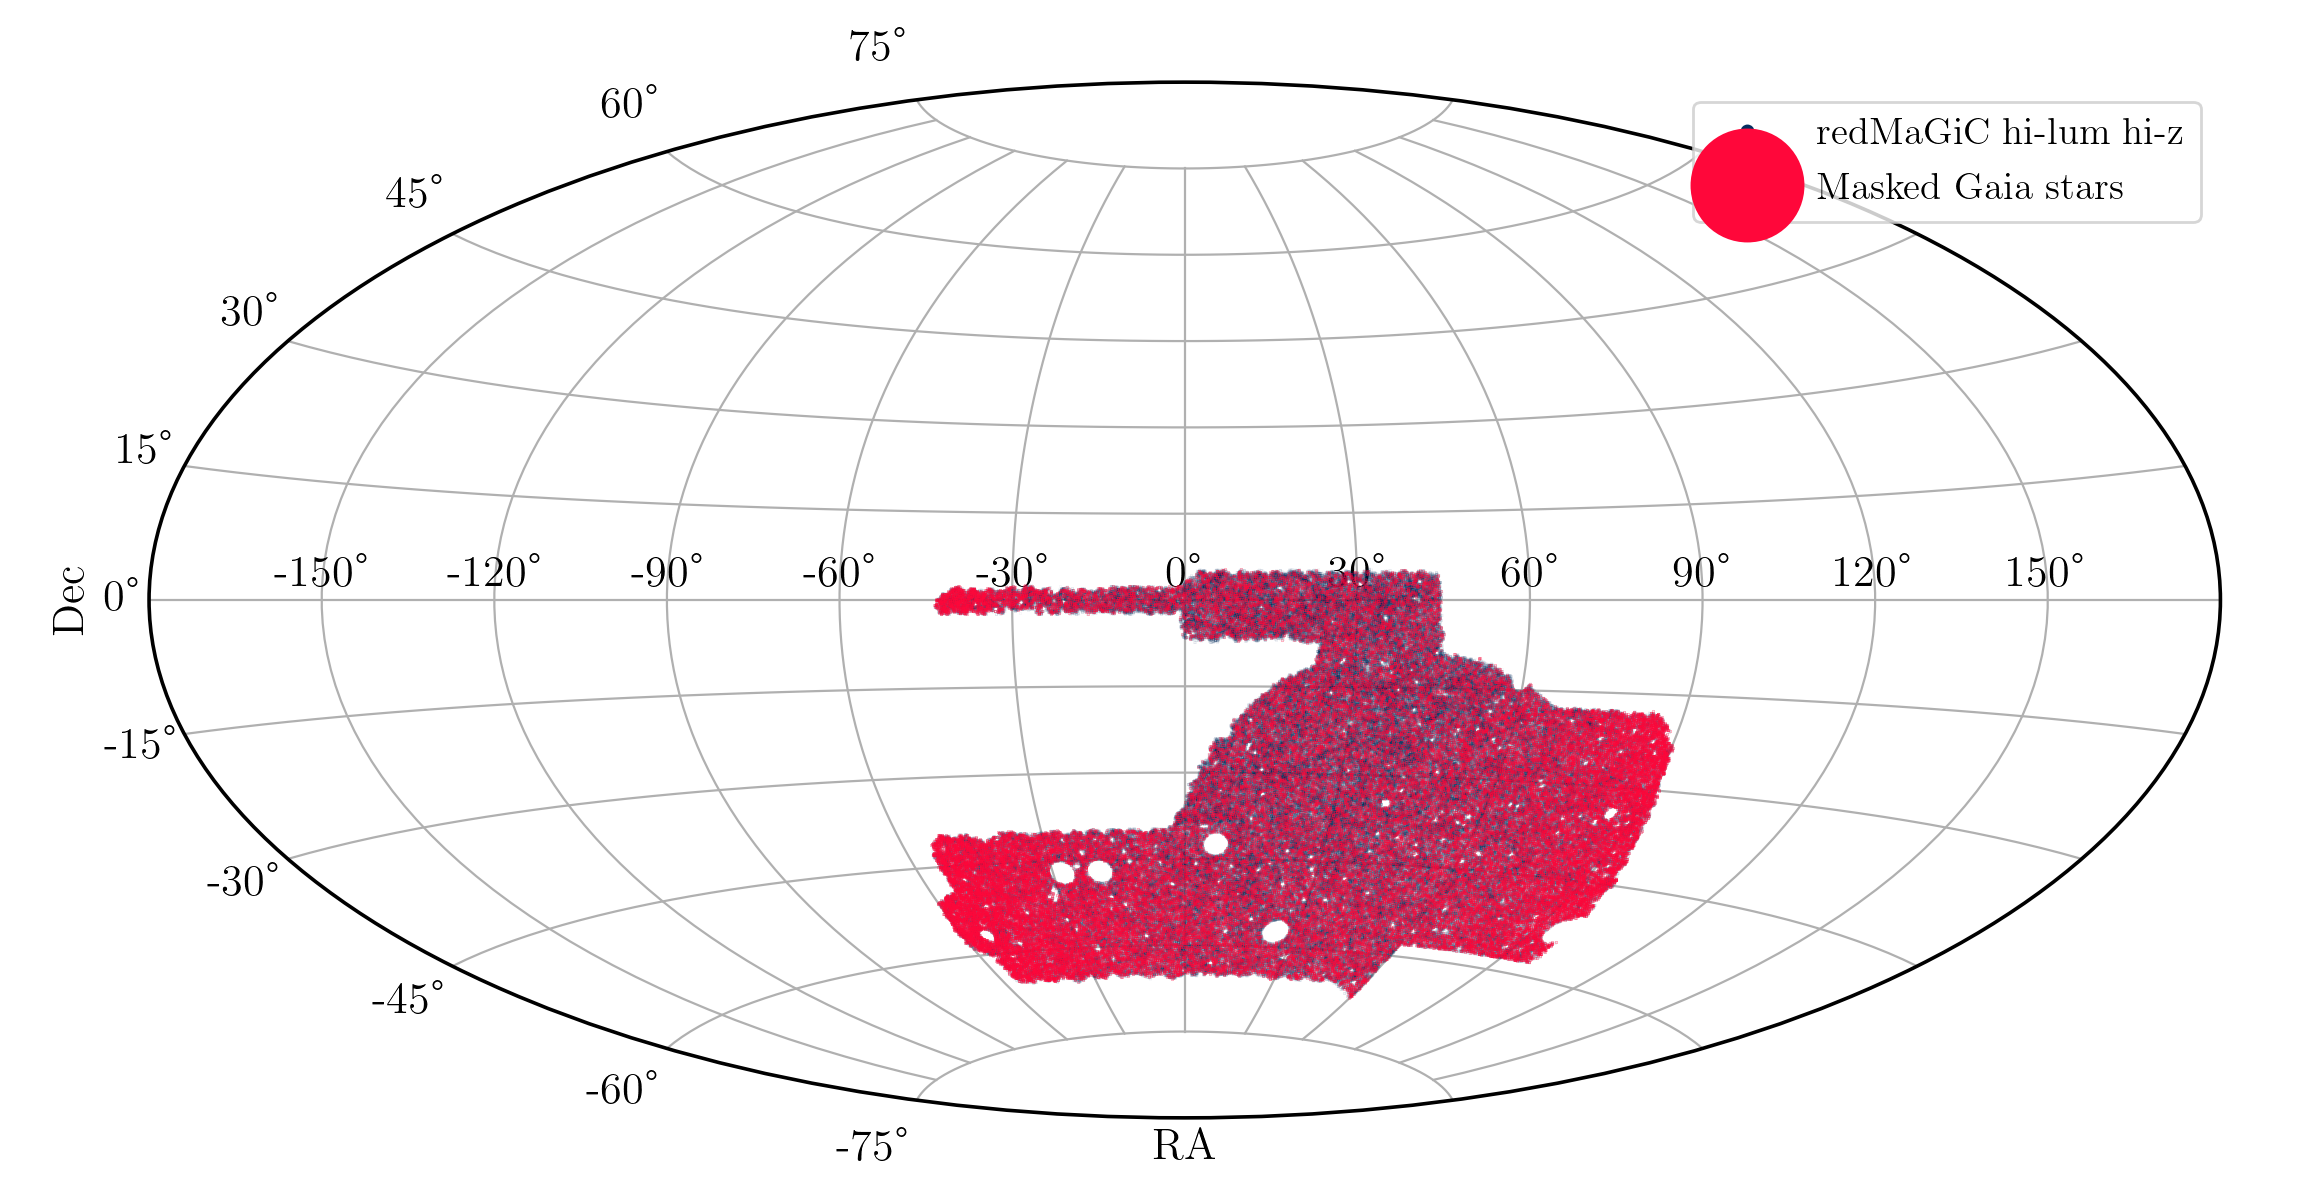
\includegraphics[width=0.75\textwidth]{figures_update2/masked_gaia_redmagic_overlap_aitoff.png}
\caption{Sky coverage of two catalogs used in this analysis: Gaia DR3 (foreground, red points) and the high-luminosity high-redshift redMaGiC 
 galaxy catalog (background, blue points). Sorry for the cartoonishly large Gaia star marker.}
\label{fig:gaiaoverlap}
\end{center}
\end{figure}

Random galaxy catalogs are not provided for either GWSLC-2 or Gaia DR3. To be able to calculate all terms in Equation \ref{eqn:xi_estimator}, I generate random foreground catalogs these two catalogs using the method first described in Update 1, Section \ref{sec:code:randoms} and corrected below. 

After all catalog joining, selections and survey masking operations, there remain: 
\begin{itemize}
\item 169,605 galaxies in the Gaia DR3 star catalog,
\item XXX galaxies in the Gaia random catalog, 
\item XXX galaxies in the GWSLC-2 catalog, 
\item and XXX galaxies in the GWSLC-2 random catalog.
\end{itemize}

% trained using the final GAMA-II spectroscopic data.


%%%%%%%%%%%%%%%%%%%%%%%%%
%%%
%%% SECTION: CODE FLOW
%%%
%%%%%%%%%%%%%%%%%%%%%%%%%

\section{Code fixes and improvements}\label{sec:code}

As stated above, there were a couple of bugs in the codebase

\subsection{Catalog processing}\label{sec:code:catalogs}

\subsubsection{Creating HEALPix survey masks}\label{sec:code:healpix}

%\begin{figure}
%\begin{center}
%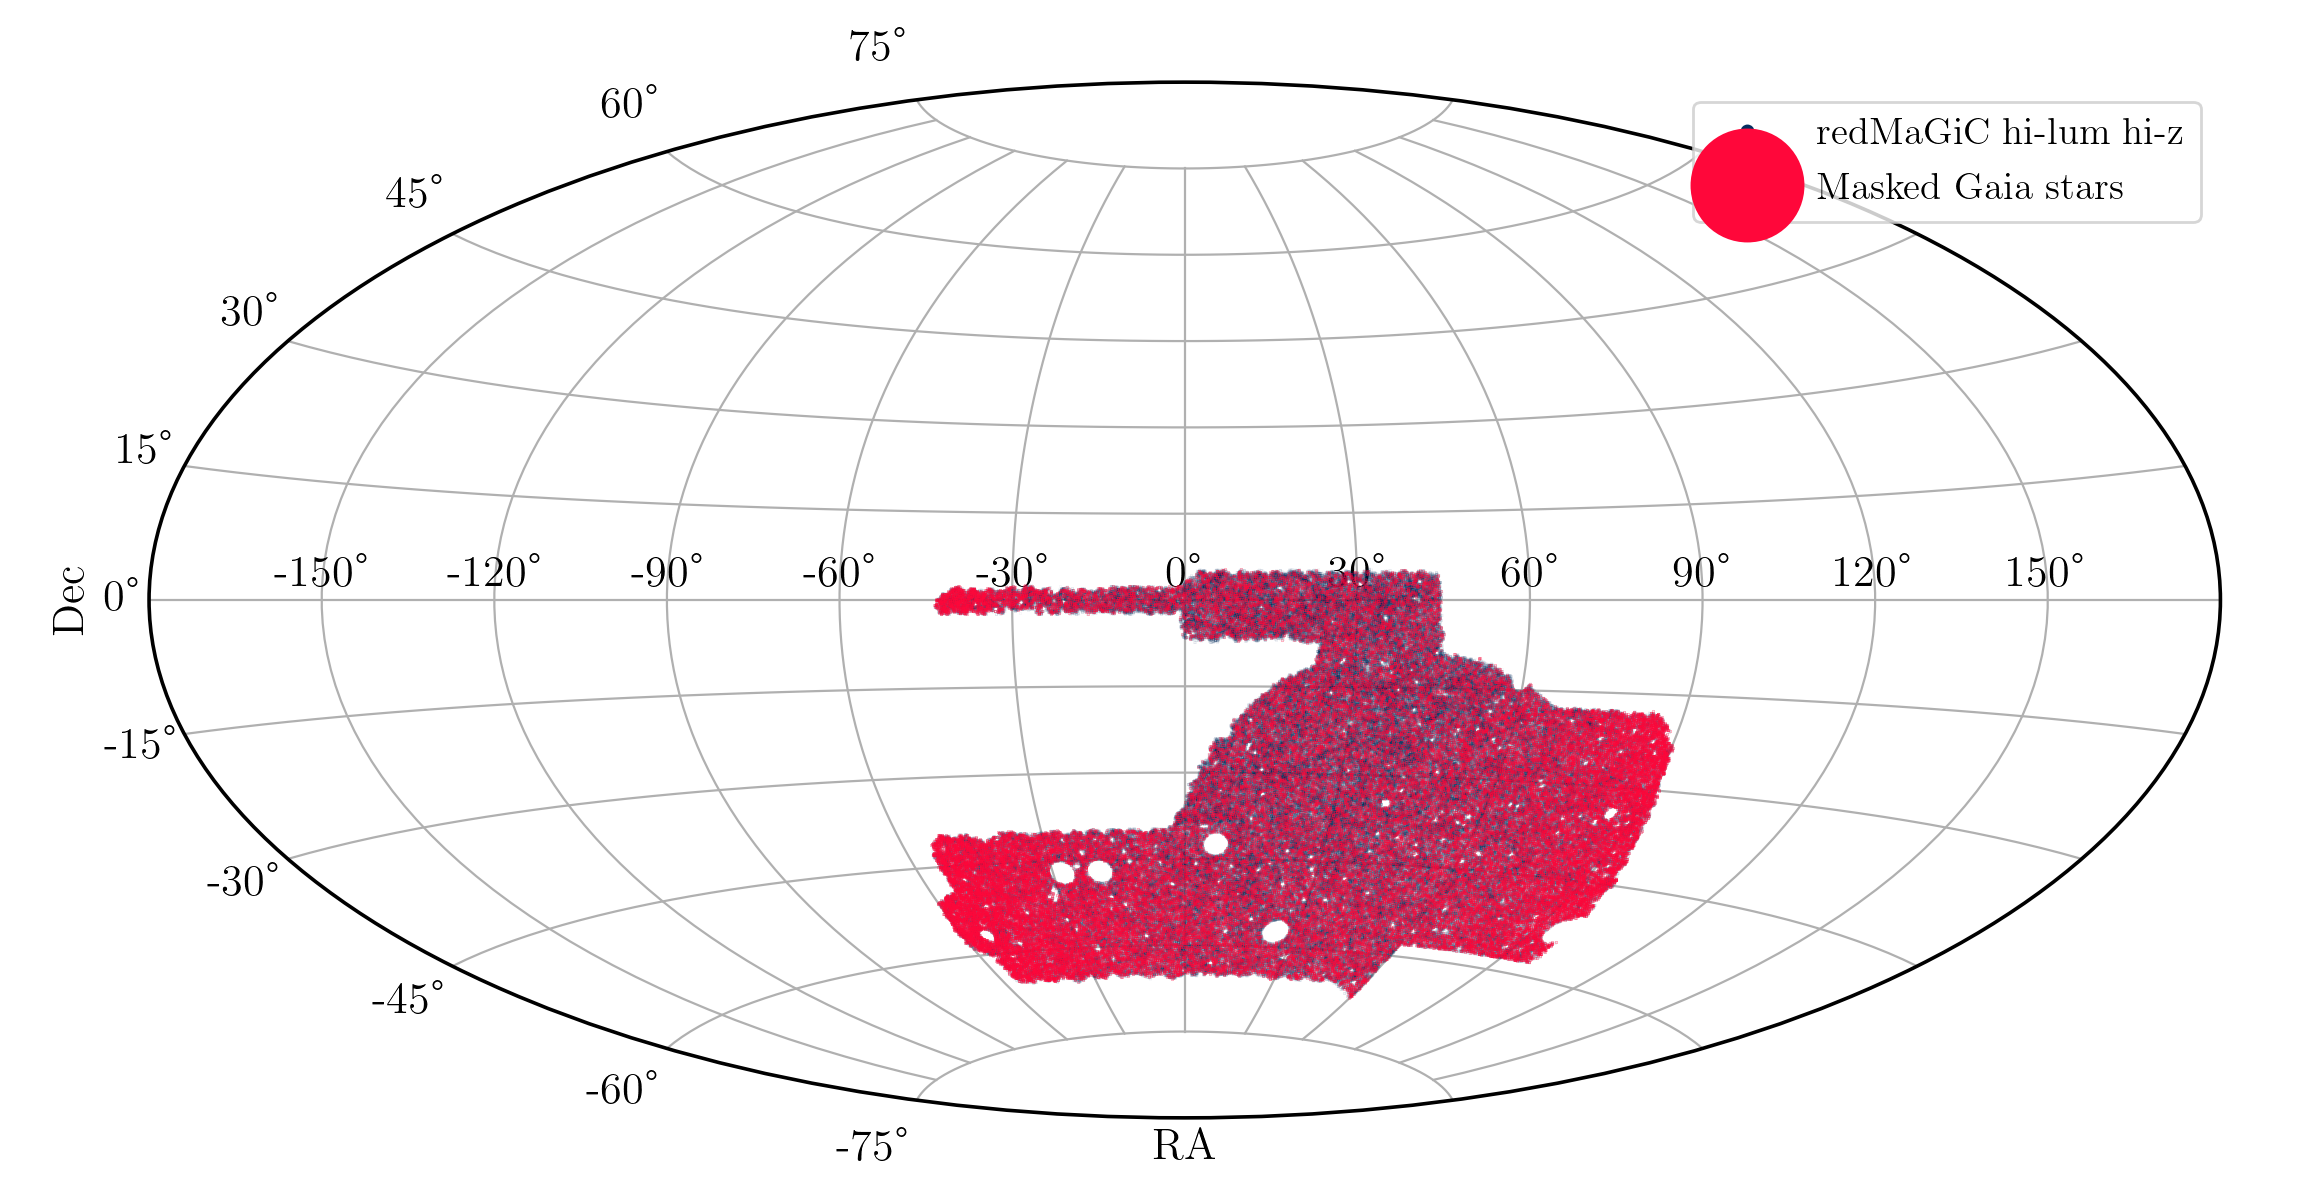
\includegraphics[width=0.75\textwidth]{figures_update2/masked_gaia_redmagic_overlap_aitoff.png}
%\caption{Color-redshift relation for the two redMaGiC catalogs (high density and high-luminosity high-redshift). Sorry for the cartoonishly large Gaia star marker}
%\label{fig:colorredshift}
%\end{center}
%\end{figure}
 

\subsubsection{Creating random catalogs}\label{sec:code:randoms}

As I described in the first update, for cases where random catalogs are not available, I developed a class called FgRandom (defined in \texttt{fg\_random.py}). In the first release, FgRandom used a seeded random number generator and the survey mask's HEALPix \texttt{NSIDE} parameter to randomly select HEALPixels and converting those to RA, Dec using the HEALPy library's \texttt{pix2ang()} function. 

An example of a random catalog generated with the original version FgRandom is shown in the top panel of Figure \ref{fig:overlap3}. I originally stated that the moir\'{e} effect was an artifact of projection and not present in the catalog itself. However, it never quite sat right with me, and my original statement turned out \textit{not} to be true! 


\begin{figure}
    \begin{center}
    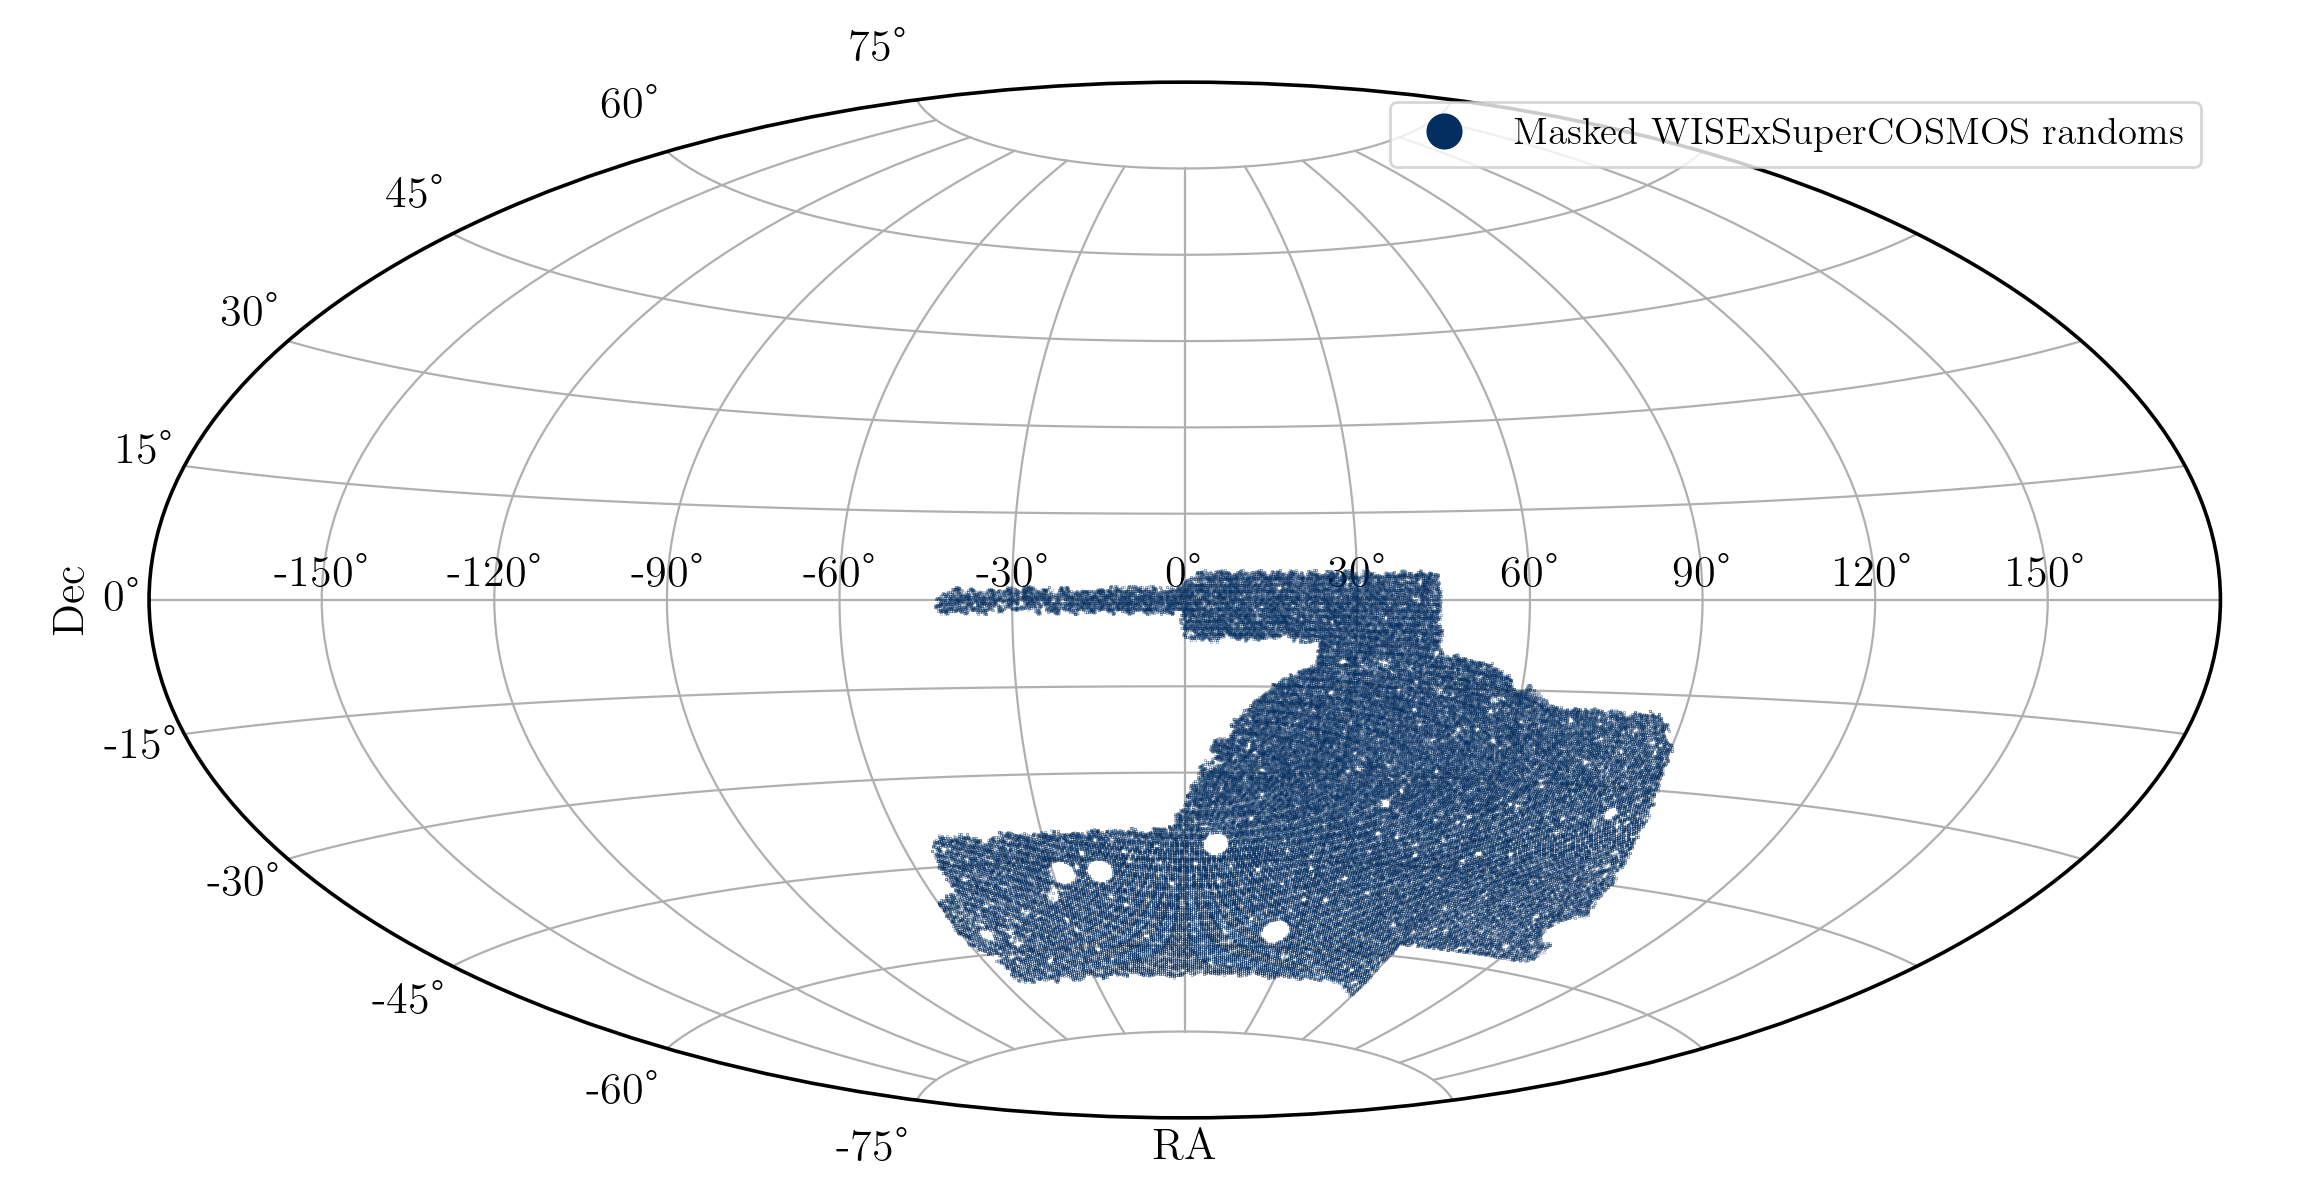
\includegraphics[width=0.65\textwidth]{figures/masked_scos_randoms_aitoff.png}\\
    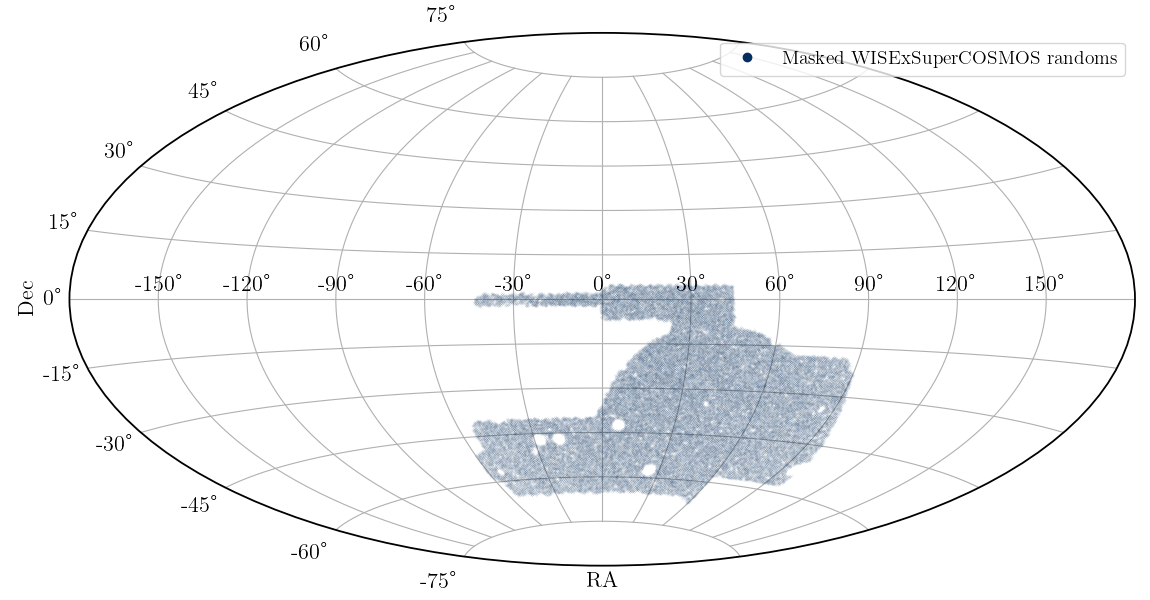
\includegraphics[width=0.65\textwidth]{figures_update2/double_masked_scos_randoms_aitoff.png}
    \caption{Sky coverage of a masked random galaxy catalog generated with two versions of FgRandom. The top panel shows the fall 2023 version, which calculated ($\alpha,\, \delta$) from randomly sampled HEALPix pixels. The bottom panel shows the result of sampling ($\alpha,\, \delta$) from a uniform distribution. The moir\'{e} pattern noticeable in the top panel is absent in the bottom panel.} 
    \label{fig:overlap3}
    \end{center}
 \end{figure}

\subsubsection{Adding photometry to random background galaxy catalogs}\label{sec:code:photom}

The redMaGiC catalogs (both real and random) have positions and redshifts, but not magnitudes. To obtain 
colors for the real catalogs, I join them with their counterparts in the Y3 GOLD catalog on the 
\texttt{COADD\_OBJECT\_ID} parameter. To do the same for the random galaxy catalogs, these objects were originally assigned photometry from the Y3 GOLD catalog randomly, with no regard for redshift. Concerned that this might introduce systematic error, I implemented redshift-based matching of random galaxies. The steps of the algorithm are relatively simple:

\begin{enumerate}
\item Generate some number of redshift bins (I chose seventeen) and digitize the photometry and random-galaxy catalogs accordingly. 
\item For each redshift bin, generate an array of random integers with as many entries as there are random galaxies in this bin and with an upper limit of the number of photometry galaxies in this bin. 
\item Assign the $g$, $r$, $i$, $z$ magnitudes of galaxies in the photometry catalog to the corresponding entries in the random-galaxy catalog elementwise.
\end{enumerate}

The result is shown in Figure \ref{fig:colormag}. Note that the photometry catalogs used for this procedure are the color-augmented redMaGiC galaxy catalogs, not the full Y3 GOLD catalog. Using the full Y3 GOLD catalog produces a mismatch in colors, which is attributable to the fact that the redMaGiC galaxies are not a representative sample!  

\begin{figure}%  figure placement: here, top, bottom, or page
   \centering
   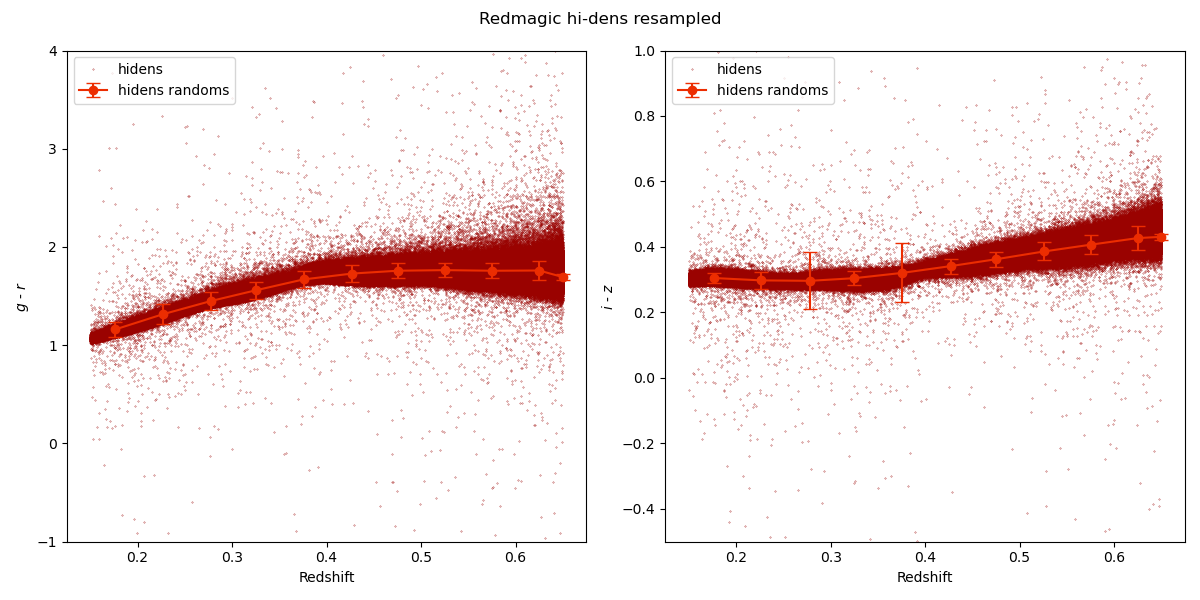
\includegraphics[width=0.65\textwidth]{figures_update2/color_redshift_redmagic_hidens_resamp.png}\\
   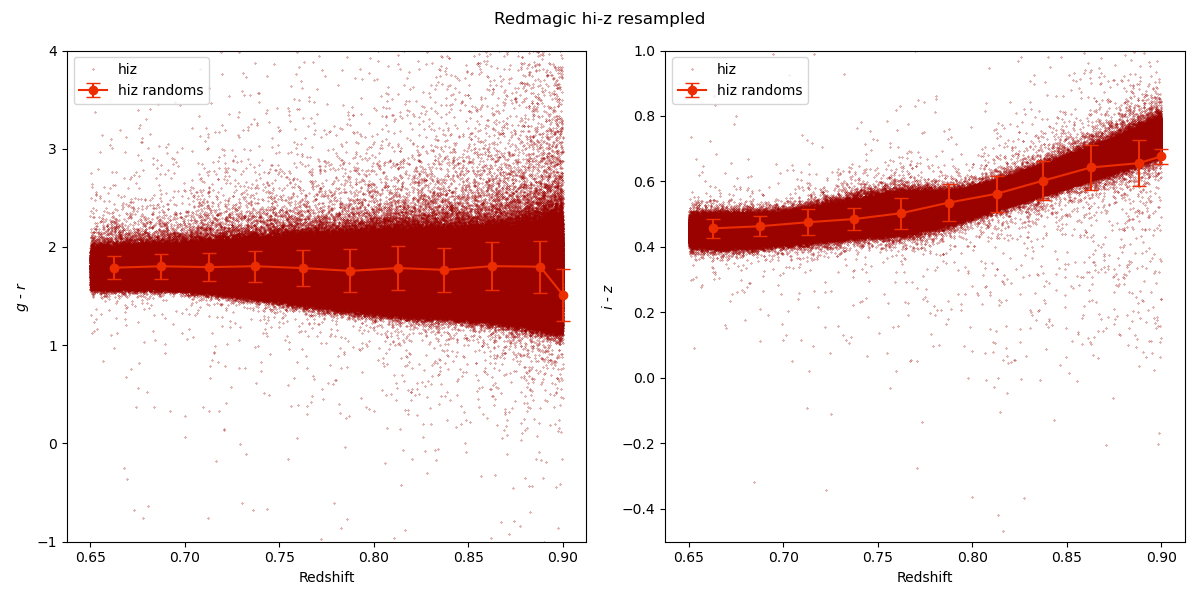
\includegraphics[width=0.65\textwidth]{figures_update2/color_redshift_redmagic_hiz_resamp.png}
   \caption{Color-redshift relation for the two redMaGiC catalogs (shown as small, dark red points) and the random galaxy catalogs (shown as large, bright red points connected by a solid line). The top row of figures shows the high density galaxy sample, the bottom row shows the high-luminosity high-redshift sample. In all cases, random galaxies' colors XXX fully overlap? are in excellent overlap with? XXX the real galaxy colors.}
   \label{fig:colormag}
\end{figure}


%%%%%%%%%%%%%%%%%%%%%%%%%
%%%
%%% SECTION: CALCULATION FLOW
%%%
%%%%%%%%%%%%%%%%%%%%%%%%%

\subsection{Extinction and correlation calculation}
As elsewhere, the correlation calculation code takes a modular approach, separating the calculation into distinct classes and functions. The code uses \texttt{TreeCorr} for the actual correlation computations and relies on a series of YAML configuration files to specify parameters, allowing for a high level of customization and reuse.

\subsubsection{Extinction models}
Models for dust-grain-induced reddening are generated with the \texttt{extinction} Python package\footnote{\url{https://extinction.readthedocs.io/en/latest/index.html}}; allowed options are \texttt{calzetti00}, \texttt{fm07}, \texttt{odonnell94}, and \texttt{fitzgerald99}. 

The \texttt{extinction} models require that wavelengths at which to compute the extinction be specified. The Virtual Observatory's Filter Profile Service provides reference wavelengths for the DECam filter set, which are shown in Table \ref{tab:filters}. I chose to calculate the extinction at the reference wavelength $\lambda_{\rm ref}$ of each filter, as it splits the difference between the other two measures. The \texttt{extinction} models also require values of $R_V$ and/or $A_V$ to be set. Values of $R_V$ in the literature fluctuate significantly from galaxy to galaxy (possibly redshift as well), and changing $R_V$ changes the extinction profiles. In the absence of a compelling reason to do otherwise, I used the default values of $R_V = 3.1$ (Milky Way-type dust) and $A_V = 1$ in my calculations. 

Model extinctions in the DECam bandpasses are reproduced below (these are identical to Update \#1): 
\small
\begin{verbatim}
wavelengths = np.array([3814.33, 4808.49, 6417.65, 7814.58, 9168.85]

# Calzetti 
extinction.calzetti00(wavelengths, 1, 3.1)
array([1.54676056, 1.19281617, 0.79717052, 0.54869537, 0.38008871])

# FM07
extinction.fm07(wavelengths, 1)
array([1.48101852, 1.19140088, 0.79964378, 0.57071627, 0.42573283])

# O'Donnell 1994
extinction.odonnell94(wavelengths, 1, 3.1)
array([1.47801728, 1.19824809, 0.83241072, 0.63597929, 0.46457349])

# CCM 89
extinction.ccm89(wavelengths, 1, 3.1)
array([1.51762325, 1.18103986, 0.8402129 , 0.62463243, 0.46457349])
\end{verbatim}

\normalsize

\begin{comment}
keep = (cat['mof_flags']==0) & (cat[`flags_badregion']==0) & \
	(cat[`mof_flux_g']>0) & (cat[`mof_flux_r']>0) & \
	(cat[`mof_flux_i']>0) & (cat[`mof_flux_z']>0) & \
          (bg_rmz['ZREDMAGIC']>zmin)

\end{comment}

\begin{table}
    \centering
    \begin{tabular}{|c|c|c|c|}
        \hline
        Filter & $\lambda_{\rm ref}$ & $\lambda_{\rm mean}$ & $\lambda_{\rm eff}$ \\
        \hline
        u & 3814.33 & 3821.68 & 3856.88 \\
        \hline
        g & 4808.49 & 4862.24 & 4769.90 \\
        \hline
        r & 6417.65 & 6460.63 & 6370.44 \\
        \hline
        i & 7814.58 & 7850.77 & 7774.30 \\
        \hline
        z & 9168.85 & 9199.28 & 9154.88 \\
        \hline
    \end{tabular}
    \caption{Reference wavelengths for the DECam filters used in this analysis. The $u$ filter is included for reference only, as the Y3GOLD catalog does not provide $u$-band magnitudes.}
    \label{tab:filters}
\end{table}


%%%%%%%%%%%%%%%%%%%%%%%%%
%%%
%%% SECTION: INITIAL RESULTS
%%%
%%%%%%%%%%%%%%%%%%%%%%%%%

\section{Updated Results}\label{sec:results}

Figures and tables in this section summarize the results of the $A_V$ estimation with the the two redMaGiC galaxy catalogs and the cross-correlation with galaxy counts in WISExSCOS. The number of redshift bins for the $A_V$ estimator calculation were chosen to balance bias and variance in the results. Five redshift slices were used for the high-luminosity, high-redshift redMaGiC sample, and fifteen redshift slices for the high-density redMaGiC sample. 

Where relevant and for ease of comparison, extinction profiles calculated with a previous generation of code and the code current as of March 2024 are juxtaposed.

\subsection{Extinction profiles}\label{sec:results:profiles}

The principal result of this analysis, extinction profiles for the WISExSCOS-redMaGiC cross-correlations, is shown in Figure \ref{fig:profile_zbins}. 


Lan \& Mo (\href{https://iopscience.iop.org/article/10.3847/1538-4357/aadc08}{2018}) and Zhu et al~(\href{https://iopscience.iop.org/article/10.1088/0004-637X/815/1/48}{2014}) show that star-forming galaxies are not the only ones for which we might expect to see large halos of dust. Figure \ref{fig:literature} implies that luminous red galaxies also possess an extended, denser CGM halo. To test this with our own sample, I cross-correlated a low-redshift subset ($z < 0.45$) of the redMaGiC high-density sample with reddening of the high-luminosity, high-redshift sample. The resulting extinction profile is shown in Figure \ref{fig:lrg_halo} and seems to confirm the existence of extended halos of cool, dense gas around LRGs. 

\begin{figure} %  figure placement: here, top, bottom, or page
   \centering
   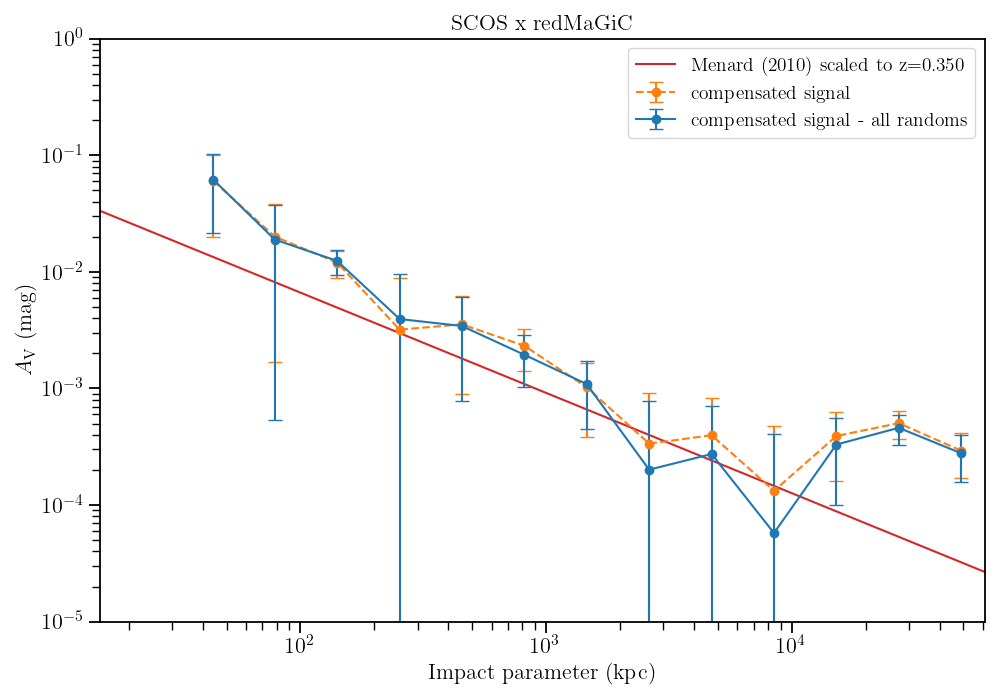
\includegraphics[width=0.65\textwidth]{figures_update2/compensated_LRG_dust_correlation_calzetti00_9bins_figure.png}
   \caption{Extinction profile of luminous red galaxies, selected from the redMaGiC high-density sample, with $z<0.45$. The redMaGiC high-luminosity high-redshift sample is used as a background catalog and $A_V$ is calculated in 9 redshift bins.}
   \label{fig:lrg_halo}
\end{figure}


As before, I explored the use of the different dust models available in the \texttt{extinction} package; $A_V$ profiles calculated using redMaGiC high-redshift galaxies and three different dust models are shown in Figure \ref{fig:profile_dustmodels}. There do not appear to be any significant differences (within error bars) between the available models, suggesting that the extinction profile isn't attributable to a fluke in a particular model. 

\begin{figure} %  figure placement: here, top, bottom, or page
   \centering
   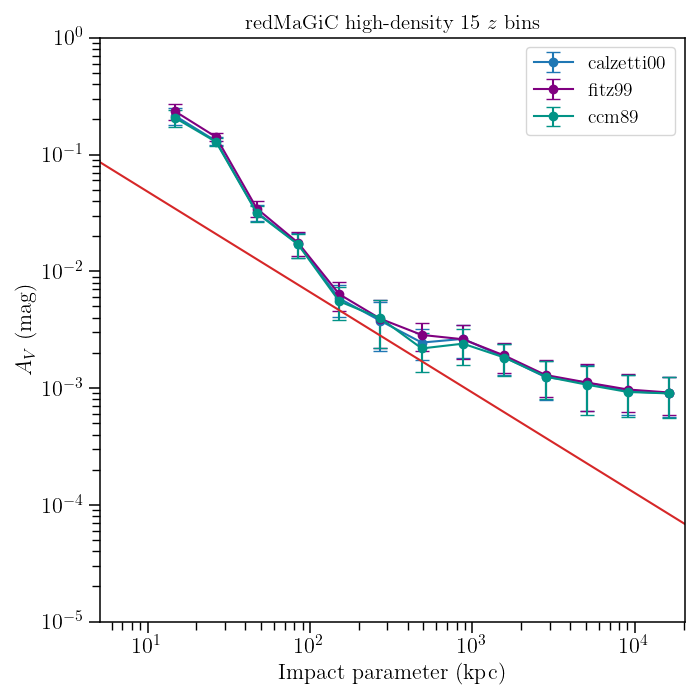
\includegraphics[width=0.65\textwidth]{figures_update2/Calzetti_vs_CCM89_vs_Fitz99.png} 
   \caption{RedMaGiC high-redshift sample extinction profiles with \av calculated in four redshift bins and with three different extinction models: \texttt{calzetti00} (light blue), \texttt{ccm89} (purple), and \texttt{fm07} (teal).}
   \label{fig:profile_dustmodels}
\end{figure}


\subsection{Sanity checks and tests}

\begin{figure} %  figure placement: here, top, bottom, or page
   \centering
   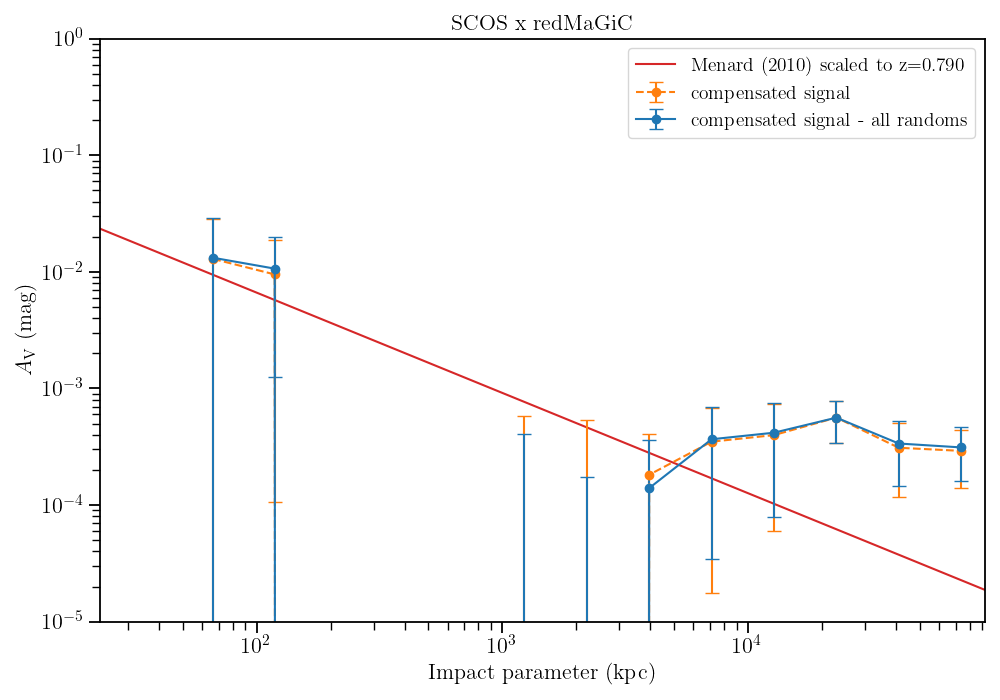
\includegraphics[width=5in]{figures_update2/compensated_lowz_bg_x_hiz_fg.png} 
   \caption{Null test: extinction profile resulting from cross-correlating a ``foreground'' sample of redMaGiC hi-z galaxies ($z > 0.65$) with reddening of actual foreground galaxies with $z<0.45$ taken from the high-density sample. Excess around 200 kpc and at $r > 10 Mpc$ are noticeable; otherwise, the curve is consistent with zero.}
   \label{fig:null_profile}
\end{figure}

\begin{figure} %  figure placement: here, top, bottom, or page
   \centering
   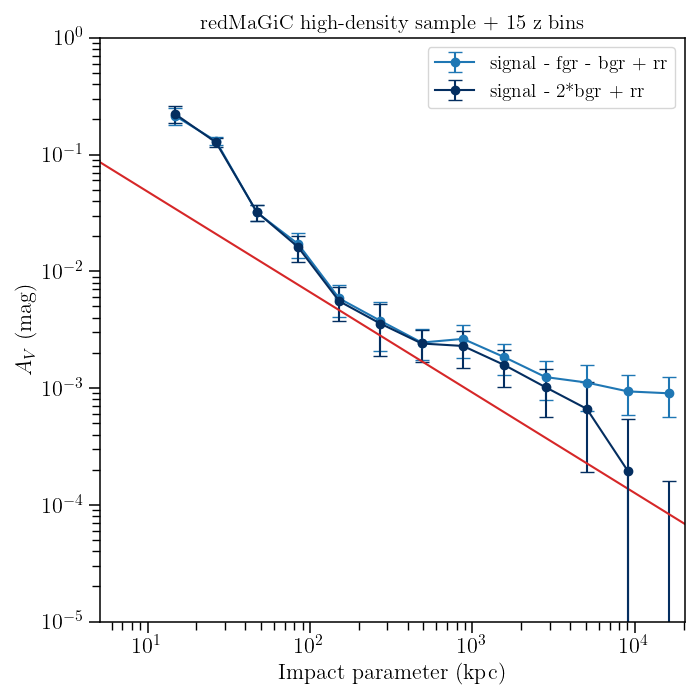
\includegraphics[width=0.45\textwidth]{figures_update2/updated_fgr_vs_not_profile.png} 
   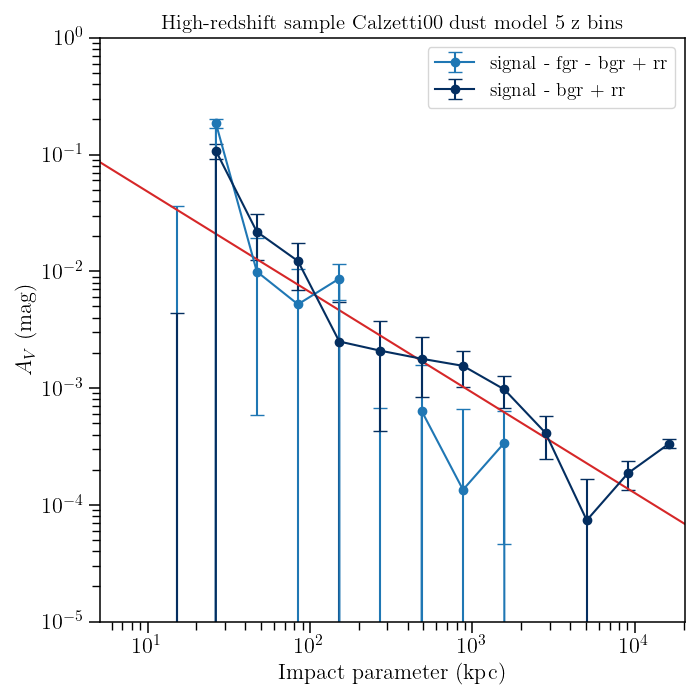
\includegraphics[width=0.45\textwidth]{figures/fgr_vs_not_profile.png} 
   \caption{Extinction profiles, with and without subtraction of the random-foreground real-background cross-correlation signal. The fully random-subtracted galaxy-\av correlations are shown in teal; the correlation without foreground random subtractions are shown in blue. An extinction profile calculated with a modified $A_V$ estimator is shown in dark blue in the left panel.}
   \label{fig:fgr_vs_not}
\end{figure}

A sharp change in the magnitude of the extinction at 200-400 kpc is visible in Figures \ref{fig:extinction}--\ref{fig:profile_dustmodels}; moreover, at high impact parameters the random subtraction is \textit{adding} power to the high-density galaxy catalog. I considered the relative contributions of the different terms in the $\xi_{N A_V}$ estimator defined in Equation \ref{eqn:xi_estimator}. An example (high density redMaGiC, \av calculated in 8 redshift bins) is shown in the left panel of Figure \ref{fig:fgr_vs_not}. It is apparent that the random-foreground, real-background cross-correlation is driving the excess at $r > 5$ Mpc.  Without that subtraction (profile in teal and dark blue lines), the extinction falls off as one might expect. The right panel of \ref{fig:fgr_vs_not} shows a similarly odd trend for the high-redshift sample: subtracting a $R_N D_{A_V}$ component makes the signal all but vanish. 

My first thought was that my random foreground catalog algorithm must have a bug, but Figure \ref{fig:null_profile} shows that the same $R_N D_{A_V}$ issue emerges when redMaGiC randoms are used instead. To produce Figure \ref{fig:null_profile}, a high-redshift ``foreground'' catalog at $z > 0.65$ was cross-correlated with reddening of a low-redshift ``background'' catalog at $z < 0.45$. In the absence of systematic error, the extinction profile should be consistent with 0. Instead, the $R_N D_{A_V}$ subtraction introduces extra signal at high impact parameter. This suggested that rather than my foreground random algorithm being incorrect, our $\xi_{N A_V}$ estimator may be flawed. Something like a Landy-Szalay estimator provided more reasonable results for the $A_V$ profile (dark blue line, left panel of Figure \ref{fig:fgr_vs_not}). However, the LRG extinction profile of Figure \ref{fig:lrg_halo} provides a counterargument to this line of reasoning: the \textit{raw} signal displays the excess at high impact parameters, and subtraction of the $R_N D_{A_V}$ removes some of this excess. So, the cause and significance of this excess at $r > 10$ Mpc remains unclear. 



%\begin{figure}
%   \centering
%   \includegraphics[width=0.5\textwidth]{/Users/j.mccleary/Research/dusty\_halos/dusthalos/outputs/AvSpread\_10zbins/av\_redmagicAll.png}
%   \caption{Histogram of $A_V$ (the optimal estimator) as calculated in 2018 with the DES Y1 redMaGiC galaxy catalog. The ``variance'' shown is actually the average value of the maximum likelihood estimator weight (sorry).}
%   \label{fig:avold}
%\end{figure}




%%%%%%%%%%%%%%%%%%%%%%%%%
%%%
%%% SECTION: NEXT STEPS
%%%
%%%%%%%%%%%%%%%%%%%%%%%%%
\section{Next steps and open questions}\label{sec:next_steps}

There are a few low-level tasks to knock out.  

\begin{itemize}
\item I need to merge my fork of \texttt{dusthalos} into Eric's original \texttt{dusthalos} repository!  
\item Measuring the extinction around GAIA stars is an easy and obvious null test that I should do again.
\item Fixing the variances on the TreeCorr correlations, since we know the defaults are too small.
\item Re-examine whether the Milky Way defaults for $R_V$, $A_V$ I used in the extinction models are appropriate for our galaxy samples.
\item Given some of the ambiguity surrounding random-foreground subtraction, it might be worthwhile to implement redshift-based matching of randoms to photometry catalogs.
\item There is a little bit of additional code development to do, such as generalizing the magnitude column names in input catalogs. 
\end{itemize}

Fundamentally, we are aiming to say something about the physics of dust and the larger galaxy environment; the following analyses could help us to that end.

\begin{enumerate}
\item Segregating galaxies by type (red vs. blue) informs models of differences in the larger-scale environments these galaxies inhabit. This is an easy test that we could carry out with the data we already have. 
\item Evaluating $A_V < 50$ kpc as a function of star formation provides an even more direct test of the connection between galaxy disks and their halos. 
\item I would like to figure out a way to get a surface dust mass as a function of radius from the galaxy. Analyzing the eBOSS galaxy sample in Lan \& Mo (2018) would be an intermediate step, but it would be nice to have something more general. \label{item:a}
\item Fitting some kind of halo model to our extinction profiles would also be cool. I don't know how to implement it, but I think it would be very illuminating to connect halo mass with dust abundance and extent. \label{item:b}
\item Proving that our estimator can recover a known quantity of dust would be a really good cross-check of our methods. Analyzing the outputs of IllustrisTNG galaxies, which include dust, could be a way to do this. \label{item:c}
\end{enumerate} 

The first two items on this list are quite simple to implement; the others are more more involved (meaning I don't know how to do them yet!). Conducting analyses \ref{item:a} and \ref{item:b} would provide a good excuse to reach out to our old friend Brandon Hensley, who doubtless knows the best way to go from extinction to some sort of physical model. For analysis \ref{item:c}, Figure \ref{fig:tng} shows that this is at least possible in theory. I'm sure I can figure it out (or put a student on it!). 

Before publishing our dust extinction results, I would like to expand this analysis to more catalogs. Doing so heads off any criticism about relying solely on DES data while also allowing us to conduct the tests above:

\begin{itemize}
\item The COSMOS catalog has blue-band magnitudes and excellent redshifts; the sky area (and thus sample size) is relatively small, but building foreground and background catalogs from COSMOS could be worth the effort, as the blue bandpasses are especially sensitive to dust extinction. 
\item Using the GALEX-SDSS-WISE Legacy Catalog as a foreground has the advantage of providing star formation rates, enabling an examination of extinction as a function of SFR. 
\item Using the DES MAGLIM catalog would vastly increase the number of galaxies available for reddening analysis. I could then reevaluate some of the odd trends evident in the high-redshift redMaGiC sample, namely, a extinction profile that disappears as $A_V$ becomes less biased.
\item The most powerful alternative catalog would be the eBOSS SDSS catalog, which has millions of galaxies, lots of blue photometry, and would allow us to reproduce the spectroscopy-based Lan \& Mo result in extinction. 
\end{itemize} 

Moving to open questions, I do wonder what is happening with those WISExSCOS/redMaGiC high-redshift measurements, particularly since the detection of the LRG extinction profile is unambiguous. Perhaps the combination of WISExSCOS and redMaGiC does not have enough constraining power by itself: the WISE catalog is comparatively thin, with a few hundred thousand objects, while the low-redshift high-density redMaGiC catalog has 630,300 galaxies. I may try relaxing the WISExSCOS redshift cut to include more galaxies. My speculation is that the ``extinction'' profile we saw with $n_{zbins} = 2$ was actually the non-zero mean value of an $A_V$ estimated in too few redshift bins. 

The question of foreground-random real-background cross-correlation is also puzzling me. At first, I believed the profile obtained with the Landry-Szaly-style estimators in Figure \ref{fig:fgr_vs_not} more than the fully-subtracted model. The reddening that emerged at high impact parameters after foreground subtraction in the hi-$z$ foreground, low-$z$ background correlation (Figure \ref{fig:null_profile}) confirmed my suspicion that $\xi_{A_V}$ shouldn't include the $R_N\,D_{A_V}$ term. However, foreground subtraction in Figure \ref{fig:lrg_halo} actually removes the extra reddening at high impact parameter. So, now I am just puzzled. If you have insights or suggestion, I am eager to hear them! 

Before too much time passes, we should also strategize about what to put in the paper\footnote{I am in favor of publishing a few smaller papers rather than one 50-page behemoth.}! Eric mentioned UV studies, and Jim had been planning a dust emission study for a while. Are either of these still in progress? Before the break, Eric and I were exploring the decomposition of the dust model into a few orthogonal axes. I have decided to abandon that line of inquiry in favor of focusing on the results we have, or can easily obtain, and connecting those to models of circumgalactic dust. If this project has legs, an orthogonal decomposition of the extinction vector would make a cool follow-up project. 


%%%%%%%%%%%%%%%%%%%%%%%%%
%%%
%%% SECTION: Conference Abstract
%%%
%%%%%%%%%%%%%%%%%%%%%%%%%

\section{Conference abstract}\label{sec:abstract}

I will be presenting a talk at ``The Physics and Impact of Astrophysical Dust: from Star Formation through Cosmology,'' an Aspen Center for Physics Winter Conference from March 3--8th. 

\textbf{Title}: 
New Evidence for Megaparsec-scale Dust Using Maximum Likelihood Estimation

\textbf{Abstract}: 
One of the more surprising astrophysical discoveries of the last decade has been an anomalous reddening of quasars consistent with dust halos (and associated large-scale structure) at cosmological scales. While this finding of extended dust halos has been confirmed several times, I will present a test of this result from a new angle: the use of maximum-likelihood formalism to construct an ``optimal estimator" for reddening of galaxy colors by dust grains. By correlating the presence of a foreground galaxy with the excess (non-cosmological) reddening of a background galaxy, I find fresh evidence for the existence of megaparsec-scale dust, transitioning from the one- to two-halo regime at scales of 100-300 kpc. While the initial analysis used the redMaGiC catalog of luminous red galaxies -- notable for its tight dispersion in color and its well-constrained photometric redshifts -- as a background sample, the result appears robust to multiple foreground-background galaxy catalog combinations. I will present an overview of our findings and outline our plans to search for sub-millimeter emission from the extended dust halos in our galaxy sample. 

\appendix
\section{Catalog prep configuration file}\label{appdx:cat_config}
\footnotesize
\begin{verbatim}
################################################################################
#                            CONFIGURATION FILE                               #
################################################################################

# Description:
# This configuration file allows you to customize the settings for
# cat_prep_runner.py

# General Settings:
# -----------------
paths:
  # general path for catalogs
  catalog_path: `/work/mccleary_group/dusty_halos/catalogs'
  # Where to save outputs
  output_path: `/work/mccleary_group/dusty_halos/catalogs/prep_cat_output'

#
# Input catalogs and masks:
# -----------------

background_catalog:
  # Where is it? Leave blank or commented out to use default
  path:
  filename: `y3a2_gold2.2.1_redmagic_highlum_highz.fits'
  # nickname for table if we are matching to another catalog
  tabname: `redmagic_hiz'
  # WCS frame
  coordframe: `icrs'
  # RA/Dec units
  coord_units: `deg'
  # RA/Dec column names
  ra_tag: `ra'
  dec_tag: `dec'
  # Name for filtered (possibly joined) output catalog
  output_name: `rmz_highlum_hiz_MOF.fits'
  # Are we matching? Uncomment fields below if true!
  match:
    # Set the path to catalog to be matched
    path: `/work/mccleary_group/dusty_halos/catalogs'
    # Name of catalog file
    filename: `des_y3_gold_MOF_highpurity_gals.fits'
    # Should be `kw', `coordinates', or `random'
    match_type: `kw'
    # If kw matching, specify
    match_kw: `coadd_object_id'
    # nickname for table
    tabname: `y3_GOLD'

background_mask:
  # Where is it? Leave blank or commented out to use default paths
  path:
  # What is it called?
  filename: `y3_gold_2.2.1_RING_joint_redmagic_v0.5.1_wide_maglim_v2.2_mask.fits'

  # IMPORTANT!!! GET COORDINATE FRAME CORRECT OR MASKING WILL FAIL!
  coordframe: `icrs'
  # Is mask partial?
  partial: True

foreground_catalog:
  # Where is it?
  #path:
  # What is it called ?
  filename: `prep_cat_output/Masked_wiseScosPhotoz160708_redshift_cut.fits'
  # Name for filtered (possibly joined) output catalog
  output_name: `redmagic_highlum_hiz_MOF.fits'
  # RA, Dec names + units + coordframe
  coordframe: `galactic'
  ra_tag: `l'
  dec_tag: `b'
  coord_units: `deg'
  # output_path: `/Users/j.mccleary/Research/dusty_halos/catalogs'
  # Are we matching? Uncomment if matching
  match:

foreground_mask:
  # Where is it?
  path:
  # What is it called?
  filename: `WISExSCOSmask.fits'
  # IMPORTANT!!! GET COORDINATE FRAME CORRECT OR MASKING WILL FAIL!
  coordframe: `galactic'
  # Is mask partial? When in doubt, do not pass this argument. Code will figure it out
\end{verbatim}

\section{Correlation/Dust Calculation Configuration File}\label{appdx:dust_config}
\footnotesize
\begin{verbatim}
################################################################################
#             CONFIGURATION FILE: dust_calc_runner.py                          #
################################################################################
# -----------------
# Input catalogs
# -----------------
# cat_config: configuration file defining properties of catalog
# NOTE: for redshifts, allowable keys are use_bin_numbers, nbins, and min_z

background_catalog:
  cat_config: `configs/catalog_configs/redmagic_hiz_y3gold_joined.yaml'
  redshifts: # How to deal with redshifts
    #use_bin_numbers: True # Basically just for redmagic
    nbins: 4

background_randoms:
  cat_config: `configs/catalog_configs/redmagic_hiz_randoms.yaml'
  redshifts: # How to deal with redshifts
    #use_bin_numbers: True # Basically just for redmagic
    nbins: 4

foreground_catalog:
  cat_config: `configs/catalog_configs/WISExSCOS_cat.yaml'

foreground_randoms:
  cat_config: `configs/catalog_configs/WISExSCOS_randoms.yaml'

# -----------------
# Correlation function parameters:
# -----------------
treecorr_params:
  min_sep: 0.1
  max_sep: 200.0
  bin_size: 0.6
  sep_units: `arcmin'

# Parameters for dust model
dust_params:
  # Must be one of `fm07', `calzetti00', `ccm89', `odonnell94', `fitzpatrick99'
  model: `calzetti00'
  # Ratio of selective to total extinction
  R: 3.1
  # Extinction in V band
  A_V: 1
  # Wavelengths (spectrum) to model; should match number of bands!
  wavelengths: [4808.49, 6417.65, 7814.58, 9168.85]

# Placeholder for selecting bands; will be made a list soon
bands:

# ------------------
# Output parameters
# ------------------
# Where output files and plots will get saved
output_path: `output/hiz'
# basename or prefix for assorted files to save
output_basename: `dust_correlation_calzetti00_4zbins'
\end{verbatim}
\end{document}  